\setcounter{cuestion}{0}
\setcounter{ejerciciogeneral}{0}
\setcounter{ejercicionumero}{0}

%\booltrue{soluciones}


\section{Ejercicios}

\subsection{Cuestiones}

\begin{question}
    Ordena los siguientes elementos según el tamaño creciente
    de sus átomos y justifica la respuesta: Si, Ne, F, Mg, S, K.

    \begin{solu}
        Debemos tener en cuenta la carga nuclear y la configuración
        de valencia de cada átomo:

%        \begin{figure}[H]
%            \centering
%            \includegraphics[scale=1]{images/imagesUD2TablaPeriodica/UD2_Problemas/cuestion1}
%            %\caption{}
%            %\label{fig:}
%        \end{figure}

        \begin{center}
            % --- tabla antigua ---
            % \begin{tblr}{hlines, vlines, colspec={Q[l,m,wd=2.9cm] c c c c c c}, row{1}={bg=mybluecolour!15, font=\bfseries}, column{1}={font=\bfseries}}
                                          % & \ch{Si}               & \ch{Ne}               & \ch{F}                & \ch{Mg}          & \ch{S}                & \ch{K}           \\
                % \(Z\)                     & 14                    & 10                    & 9                     & 12               & 16                    & 19               \\
                % Configuración de valencia & \(\mathrm{3s^2\,3p^2}\) & \(\mathrm{2s^2\,2p^6}\) & \(\mathrm{2s^2\,2p^5}\) & \(\mathrm{3s^2}\) & \(\mathrm{3s^2\,3p^4}\) & \(\mathrm{4s^1}\) \\
            % \end{tblr}
            % --- tabla nueva ---
            \begin{tabular}{@{}L{2.9cm} c c c c c c@{}}
                \toprule
                 & \textbf{\ch{Si}} & \textbf{\ch{Ne}} & \textbf{\ch{F}} & \textbf{\ch{Mg}} & \textbf{\ch{S}} & \textbf{\ch{K}} \\
                \midrule
                \textbf{\(Z\)} & 14 & 10 & 9 & 12 & 16 & 19 \\[3pt]
                \textbf{Configuración de valencia} & \(\mathrm{3s^2\,3p^2}\) & \(\mathrm{2s^2\,2p^6}\) & \(\mathrm{2s^2\,2p^5}\) & \(\mathrm{3s^2}\) & \(\mathrm{3s^2\,3p^4}\) & \(\mathrm{4s^1}\) \\
                \bottomrule
            \end{tabular}
        \end{center}

        El mayor tamaño lo tiene el K, pues sus electrones de valencia
        están en la capa más alejada del núcleo (mayor número cuántico
        principal), lo que pesa más que el aumento de la carga nuclear.

        Para los elementos que están en un mismo período (Mg, Si, S), la
        capa de valencia es la misma, por lo que la comparación depende
        de la carga nuclear efectiva, \(Z_{ef} = Z - \sigma\), siendo
        \(\sigma\) el apantallamiento que ejercen los electrones internos.
        Al recorrer el período de izquierda a derecha, la carga nuclear
        \(Z\) aumenta en una unidad por cada elemento, mientras que el
        apantallamiento de los electrones internos apenas varía; por
        ello, \(Z_{ef}\) crece a lo largo del período. Cuanto mayor es
        \(Z_{ef}\), mayor es la atracción del núcleo sobre los electrones
        de valencia y menor el tamaño de la corteza electrónica. El
        mismo razonamiento se aplica a F y Ne, que pertenecen al
        período 2.
        En consecuencia, el orden creciente es el siguiente:

        \[K > Mg > Si > S > F > Ne\]
    \end{solu}
\end{question}

\begin{question}
    Razona si es cierto que un ion siempre tiene un tamaño
    menor que el del átomo correspondiente.

    \begin{solu}
        El catión tiene menor tamaño que el átomo correspondiente,
        pero el anión es más grande que su átomo.
    \end{solu}
\end{question}

\begin{question}
    Ordena los siguientes elementos químicos por su radio
    atómico: Se, Br, Kr, Rb y Sr. Determina la configuración
    electrónica del ion más estable que se puede formar
    con cada uno de estos átomos y ordena dichos iones
    según su radio.


    \begin{solu}

%        \begin{figure}[H]
%            \centering
%            \includegraphics[scale=1]{ images/imagesUD2TablaPeriodica/UD2_Problemas/cuestion3.png}
%            %\caption{}
%            %\label{fig:}
%        \end{figure}

        Tienen mayor tamaño los elementos del período 5 (Rb, Sr) que los
        del 4 (Se, Br, Kr), porque sus electrones de valencia están más
        alejados del núcleo, lo que prevalece sobre el efecto de la
        carga nuclear. Dentro de cada período, el apantallamiento
        \(\sigma\) que ejercen los electrones internos es prácticamente
        el mismo para todos los elementos, mientras que la carga
        nuclear \(Z\) aumenta con el número atómico; por ello, la carga
        nuclear efectiva \(Z_{ef} = Z - \sigma\) crece a lo largo del
        período. Cuanto mayor es \(Z_{ef}\), mayor es la atracción que
        el núcleo ejerce sobre los electrones más periféricos y menor
        el radio atómico:
        \[Rb > Sr > Se > Br > Kr\]

        Los iones más estables de estos elementos son \(\ch{Se^2-}\),
        \(\ch{Br-}\), \(\ch{Kr}\) (no forma iones estables), \(\ch{Rb+}\)
        y \(\ch{Sr^2+}\), todos con la configuración electrónica de gas
        noble del \ch{Kr}. Al tener todos ellos el mismo número de
        electrones (36) e idéntico apantallamiento, el radio del ion
        depende únicamente de la carga nuclear: cuanto mayor es \(Z\),
        mayor es \(Z_{ef}\) sobre esos 36 electrones y menor el radio
        iónico. Como \(\ch{Se^2-}\) tiene la menor carga nuclear
        (\(Z=34\)) y \(\ch{Sr^2+}\) la mayor (\(Z=38\)), el orden
        creciente de radio iónico es:
        \[\ch{Sr^2+} < \ch{Rb+} < \ch{Br-} < \ch{Se^2-}\]
    \end{solu}
\end{question}

\begin{question}
    Justifica por qué los elementos de transición de un mismo
    período tienen tamaños tan parecidos.


    \begin{solu}
        Tienen tamaños tan parecidos porque todos poseen la misma
        configuración electrónica en su capa más exterior; el electrón
        diferenciador se sitúa en una capa más interior. Por otra
        parte, su número atómico es lo suficientemente alto como
        para que no sea muy significativa la presencia de un protón
        más en el núcleo del átomo de cada elemento.
    \end{solu}

\end{question}

\begin{question}
    Indica por qué no es correcta la siguiente definición:
    «El potencial de ionización es la energía que hay que
    comunicar a un átomo para arrancarle un electrón».


    \begin{solu}
        No es correcta la afirmación porque hay que precisar que el
        átomo debe estar aislado y que el electrón ha de hallarse en
        la capa de valencia del átomo
    \end{solu}

\end{question}

\begin{question}
    ¿Cuántas energías de ionización se pueden establecer
    en el caso del aluminio?

    \begin{solu}
        Para el aluminio se pueden establecer 13 energías de ionización,
        ya que tiene 13 electrones.
    \end{solu}

\end{question}

\begin{question}
    Explica por qué el segundo potencial de ionización de
    un elemento químico tiene el mismo signo que el primero,
    y la segunda afinidad electrónica, signo contrario
    a la primera.


    \begin{solu}
        El potencial de ionización es la energía que hay que comunicar
        a un átomo en estado gaseoso para arrancarle un electrón.
        Si se trata del segundo electrón, será el segundo potencial
        de ionización y habrá que comunicarle aún más energía
        para arrancárselo.

        La afinidad electrónica, por su parte, es la energía que desprende
        el átomo en estado gaseoso cuando capta un electrón. Si se trata del segundo electrón, será la segunda afinidad electrónica, pero un átomo nunca cederá energía al captar un
        segundo electrón; por el contrario, si se quiere que suceda
        esto habrá que comunicársela. Por eso, la segunda afinidad
        electrónica siempre tiene signo contrario a la primera.

    \end{solu}

\end{question}

\begin{question}
    El litio, el sodio y el potasio son tres metales alcalinos de
    número atómico 3, 11 y 19, respectivamente. Asigna de
    manera razonada a cada uno de estos metales uno de
    los siguientes valores posibles para la energía de ionización:
    100 kcal/mol, 119 kcal/mol y 124 kcal/mol.


    \begin{solu}
        Debemos tener en cuenta la carga nuclear y la configuración
        de valencia de cada átomo:

%        \begin{figure}[H]
%            \centering
%            \includegraphics[scale=1]{ images/imagesUD2TablaPeriodica/UD2_Problemas/cuestion8.png}
%            %\caption{}
%            %\label{fig:}
%        \end{figure}

        \begin{center}
            % --- tabla antigua ---
            % \begin{tblr}{hlines, vlines, colspec={l c c c}, row{1}={bg=mybluecolour!15, font=\bfseries}, column{1}={font=\bfseries}}
                                                                   % & \ch{Li}           & \ch{Na}           & \ch{K}            \\
                % \(Z\)                                              & 3                 & 11                & 19                \\
                % Configuración de valencia                          & \(\mathrm{2s^1}\) & \(\mathrm{3s^1}\) & \(\mathrm{4s^1}\) \\
                % Energía de ionización (\unit{\kilo\calorie\per\mole}) & 124               & 119               & 100               \\
            % \end{tblr}
            % --- tabla nueva ---
            \begin{tabular}{@{}lccc@{}}
                \toprule
                 & \textbf{\ch{Li}} & \textbf{\ch{Na}} & \textbf{\ch{K}} \\
                \midrule
                \textbf{\(Z\)} & 3 & 11 & 19 \\[3pt]
                \textbf{Configuración de valencia} & \(\mathrm{2s^1}\) & \(\mathrm{3s^1}\) & \(\mathrm{4s^1}\) \\[3pt]
                \textbf{Energía de ionización (\unit{\kilo\calorie\per\mole})} & 124 & 119 & 100 \\
                \bottomrule
            \end{tabular}
        \end{center}

        La energía de ionización es la que se requiere para arrancar
        el electrón de valencia a un mol de átomos del elemento en
        estado gaseoso. Todos estos elementos tienen un único electrón
        de valencia, pero situado en capas distintas (2, 3 y 4,
        respectivamente); al ser todos alcalinos, la carga nuclear
        efectiva sobre ese electrón de valencia es similar en los tres
        (\(Z_{ef} \approx +1\), ya que el resto de electrones internos
        apantalla casi por completo el aumento de \(Z\)), por lo que el
        factor decisivo es la distancia al núcleo. Resultará más fácil
        arrancárselo al potasio, pues en su caso ese electrón se
        encuentra en una capa más alejada del núcleo que en cualquiera
        de los otros dos. En consecuencia, el potasio tiene la menor
        energía de ionización (100 kcal/mol), seguido del sodio
        (119 kcal/mol) y del litio (124 kcal/mol).


    \end{solu}

\end{question}

\begin{question}
    Ordena según el valor creciente de su primera energía
    de ionización, justificando las posibles anomalías, los
    siguientes elementos: Al, Ne, P, Mg, S y K.


    \begin{solu}
        Debemos tener en cuenta la carga nuclear y la configuración
        de valencia de cada átomo:
%        \begin{figure}[H]
%            \centering
%            \includegraphics[scale=1]{ images/imagesUD2TablaPeriodica/UD2_Problemas/cuestion9}
%            %\caption{}
%            %\label{fig:}
%        \end{figure}

        \begin{center}
            % --- tabla antigua ---
            % \begin{tblr}{hlines, vlines, colspec={Q[l,m,wd=2.9cm] c c c c c c}, row{1}={bg=mybluecolour!15, font=\bfseries}, column{1}={font=\bfseries}}
                                          % & \ch{Al}               & \ch{Ne}               & \ch{P}                & \ch{Mg}          & \ch{S}                & \ch{K}           \\
                % \(Z\)                     & 13                    & 10                    & 15                    & 12               & 16                    & 19               \\
                % Configuración de valencia & \(\mathrm{3s^2\,3p^1}\) & \(\mathrm{2s^2\,2p^6}\) & \(\mathrm{3s^2\,3p^3}\) & \(\mathrm{3s^2}\) & \(\mathrm{3s^2\,3p^4}\) & \(\mathrm{4s^1}\) \\
            % \end{tblr}
            % --- tabla nueva ---
            \begin{tabular}{@{}L{2.9cm} c c c c c c@{}}
                \toprule
                 & \textbf{\ch{Al}} & \textbf{\ch{Ne}} & \textbf{\ch{P}} & \textbf{\ch{Mg}} & \textbf{\ch{S}} & \textbf{\ch{K}} \\
                \midrule
                \textbf{\(Z\)} & 13 & 10 & 15 & 12 & 16 & 19 \\[3pt]
                \textbf{Configuración de valencia} & \(\mathrm{3s^2\,3p^1}\) & \(\mathrm{2s^2\,2p^6}\) & \(\mathrm{3s^2\,3p^3}\) & \(\mathrm{3s^2}\) & \(\mathrm{3s^2\,3p^4}\) & \(\mathrm{4s^1}\) \\
                \bottomrule
            \end{tabular}
        \end{center}
        La energía de ionización es la que se requiere para arrancar
        el electrón de valencia a un mol de átomos del elemento en
        estado gaseoso. Su valor depende de la configuración de la
        capa de valencia y, sobre todo, de la carga nuclear efectiva
        \(Z_{ef} = Z - \sigma\) que percibe el electrón de valencia:
        cuanto mayor es \(Z_{ef}\), con más fuerza lo retiene el átomo y
        mayor es su energía de ionización.
        De todos los presentes, el K es el elemento de menor energía
        de ionización, ya que tiene el electrón de valencia en la capa
        más alejada del núcleo (\(n=4\)) y solo tiene uno, muy apantallado
        por el resto de electrones internos.
        De los elementos que están en el tercer período (Mg, Al, S y P),
        el apantallamiento interno es prácticamente el mismo para todos
        ellos, de modo que \(Z_{ef}\) aumenta con \(Z\) a lo largo del
        período; el Mg es el que tiene menor energía de ionización,
        pues es el que tiene menos protones en su núcleo (menor \(Z\) y,
        por tanto, menor \(Z_{ef}\)). Le sigue el Al. El S tiene
        un protón más en el núcleo que el P; por tanto, se podría
        pensar que su energía de ionización es mayor. No obstante,
        el P tiene estructura de semicapa cerrada (\(3p^13p^13p^1\)), una
        estructura de especial estabilidad que puede alcanzar el S si
        pierde un electrón de valencia; por este motivo, la energía de
        ionización del S es menor que la del P.
        Finalmente, el Ne es el elemento con la energía de ionización
        más alta, ya que tiene estructura de capa cerrada (es un gas
        noble) y es muy difícil que la pierda.
        75
        Sistema periódico de los elementos 2
        Unidades didácticas Química 2.º Bachillerato
        En conclusión, el orden de los elementos según su energía de
        ionización sería, de mayor a menor:
        \[Ne > P > S > Al > Mg > K\]
    \end{solu}

\end{question}

\begin{question}
    Ordena los siguientes elementos según su primer potencial
    de ionización: Br, K, Mg y S. Si atendemos a su segundo potencial de ionización, ¿estarían en el mismo orden?


    \begin{solu}

%        \begin{figure}[H]
%            \centering
%            \includegraphics[scale=1]{ images/imagesUD2TablaPeriodica/UD2_Problemas/cuestion10a.png}
%            %\caption{}
%            %\label{fig:}
%        \end{figure}
%
%        \begin{figure}[H]
%            \centering
%            \includegraphics[scale=1]{ images/imagesUD2TablaPeriodica/UD2_Problemas/cuestion10b.png}
%            %\caption{}
%            %\label{fig:}
%        \end{figure}

        La justificación reside en la configuración electrónica de la
        especie que va a perder el electrón y en la carga nuclear
        efectiva \(Z_{ef} = Z - \sigma\) que actúa sobre ese electrón.

        El Br y el S pertenecen al período 4 y al período 3
        respectivamente, mientras que el K y el Mg se encuentran en el
        mismo período que, en cada caso, el elemento con el que se
        comparan; en todos los casos, cuanto mayor es \(Z_{ef}\) sobre
        el electrón de valencia, mayor es el primer PI.
        El elemento con mayor 1.er PI es el Br, al que solo le falta un
        electrón para alcanzar la configuración de gas noble (elevada
        \(Z_{ef}\) por su posición al final del período) y que,
        por ello, tiene muy poca tendencia a perder electrones; le
        sigue el S, al que le faltan 2 electrones para tener configuración
        de gas noble. Entre estos dos elementos, el S es el que
        tiene mayor segundo PI, ya que posee estructura de semicapa
        cerrada, de especial estabilidad.

        El tercer elemento, en lo que al valor del primer PI se refiere,
        es el Mg, que solo tiene 2 electrones en su capa de valencia,
        poco apantallados frente a la \(Z_{ef}\) que ya ejerce su núcleo.
        Al perder el segundo electrón, adquiere configuración de gas
        noble; por eso, es el elemento que tiene menor segundo PI.

        El 1.er PI más bajo lo tiene el K, ya que su único electrón de
        valencia ocupa la capa \(n=4\), muy alejada del núcleo y muy
        apantallada por el resto de electrones internos (\(Z_{ef}\)
        pequeña); si lo pierde, adquiere configuración de gas noble.
        Por esta razón, es el elemento que
        tiene el segundo PI más alto.
    \end{solu}

\end{question}

\begin{question}
    Las especies H, \ch{He+} y \ch{Li\pch[2]} poseen un solo electrón.
    Razona
    cuál de ellas poseerá: a) la mayor energía de ionización;
    b) el radio más grande.


    \begin{solu}
        Consideramos la carga nuclear de estas especies:
%        \begin{figure}[H]
%            \centering
%            \includegraphics[scale=1]{images/imagesUD2TablaPeriodica/UD2_Problemas/cuestion11.png}
%            %\caption{}
%            %\label{fig:}
%        \end{figure}

        \begin{center}
            % --- tabla antigua ---
            % \begin{tblr}{hlines, vlines, colspec={l c c c}, row{1}={bg=mybluecolour!15, font=\bfseries}, column{1}={font=\bfseries}}
                      % & \ch{H} & \ch{He+} & \ch{Li\pch[2]} \\
                % \(Z\) & 1      & 2        & 3              \\
            % \end{tblr}
            % --- tabla nueva ---
            \begin{tabular}{@{}lccc@{}}
                \toprule
                 & \textbf{\ch{H}} & \textbf{\ch{He+}} & \textbf{\ch{Li\pch[2]}} \\
                \midrule
                \textbf{\(Z\)} & 1 & 2 & 3 \\
                \bottomrule
            \end{tabular}
        \end{center}
        Al tener un único electrón, no existe apantallamiento
        (\(\sigma = 0\)), por lo que la carga nuclear efectiva coincide
        con la carga nuclear real: \(Z_{ef} = Z\). Las cargas nucleares
        son \(Z=1\) para \ch{H}, \(Z=2\) para \ch{He+} y \(Z=3\) para
        \ch{Li\pch[2]}. Cuando mayor sea la carga nuclear (y, por tanto,
        \(Z_{ef}\)), mayor será la atracción
        que el núcleo ejerce sobre el electrón; en consecuencia, mayor
        será la energía de ionización y menor será el radio:

        \begin{enumerate}[label=\letraminuscula]
            \item  Energía de ionización: \ch{Li\pch[2]} \textgreater  \ch{He+} \textgreater \ch{H}
            \item Radio: \ch{Li\pch[2]} \textless \ch{He+} \textless \ch{H}
        \end{enumerate}

    \end{solu}

\end{question}

\begin{question}
    Indica si la energía que interviene en el siguiente proceso
    es la afinidad electrónica del cloro:

    \begin{equation*}
        \ch{1/2 Cl2 \gas{} + energía -> Cl-}
    \end{equation*}


    \begin{solu}
        No es la afinidad electrónica. Esta se define como la energía
        que cede el átomo del elemento cuando capta un electrón.
        Se representa mediante la ecuación:

        \begin{equation*}
            \ch{1/2 Cl2 \gas{} + \el{} -> Cl- + energía}
        \end{equation*}
    \end{solu}

\end{question}

\begin{question}
    Justifica por qué la afinidad electrónica del flúor es, en
    contra de lo que cabría esperar, menor que la del cloro.


    \begin{solu}
        Cabría esperar que la afinidad electrónica del F fuera mayor,
        ya que su carga nuclear efectiva \(Z_{ef}\) es ligeramente
        superior a la del Cl (menos capas internas que apantallen).
        Sin embargo, es más pequeña porque el electrón que capta el F
        se introduce en la capa 2, un volumen muy reducido, donde va a
        sufrir fuertes repulsiones con los demás electrones ya
        presentes en esa misma capa. Esas repulsiones electrón-electrón
        serán menos significativas en el caso del Cl, pues el electrón
        que se introduce lo hace en la capa 3, de mayor tamaño que la
        2, lo que compensa su menor \(Z_{ef}\).
    \end{solu}

\end{question}

\begin{question}
    Tanto la afinidad electrónica como la electronegatividad
    miden la tendencia de un átomo a atraer electrones.
    Explica en qué se diferencian ambas propiedades.


    \begin{solu}
        La afinidad electrónica es la energía de un proceso y se puede
        medir. Por su parte, la electronegatividad es una propiedad
        que se define, pero que no se mide de forma directa. La escala
        de electronegatividades se establece por comparación y
        no se mide en unas unidades concretas.
    \end{solu}
\end{question}

\begin{question}
    Teniendo en cuenta su electronegatividad, justifica por
    qué el hidrógeno actúa con números de oxidación +1 y -1. Ver tabla de electronegatividades de Pauling.


    \begin{solu}
        En la escala de electronegatividades (de 0 a 4), el H tiene
        una electronegatividad intermedia (2,2); por eso, cuando se
        combina con elementos más electronegativos, su estado de
        oxidación será +1, y cuando lo hace con los menos electronegativos,
        será -1.
    \end{solu}

\end{question}

\begin{question}
    El flúor es el elemento más electronegativo. ¿Por qué?
    ¿Cuál es el menos electronegativo? ¿Por qué?


    \begin{solu}
        Es el más electronegativo porque es el elemento para el cual
        la suma de PI + AE alcanza un valor mayor. Cuando se enlace
        a cualquier otro elemento de la tabla periódica, será el F el
        que lleve sobre sí los electrones del enlace.
        El elemento menos electronegativo es el Cs (no se considera
        el Fr por ser un elemento radiactivo). El Cs es el elemento
        para el cual la suma de PI + AE alcanza un valor menor. Cuando
        se una a cualquier otro elemento de la tabla periódica,
        será el Cs el que tenga menos carga electrónica de enlace
        sobre sí.
    \end{solu}

\end{question}

\begin{question}
    Dadas las siguientes configuraciones electrónicas asignadas
    a átomos en estado fundamental:

    \begin{itemize}
        \item \elconf{Na}.
        \item \elconf{F}
        \item \elconf{Ar}
    \end{itemize}

    \begin{enumerate}[label=\letraminuscula]
    \item ¿A qué elementos corresponden?
    \item ¿Cuál será el más electronegativo? ¿Por qué?
    \end{enumerate}


    \begin{solu}
        \begin{enumerate}[label=\letraminuscula]
            \item Un átomo tiene el mismo número de protones que de
            electrones, por lo que podemos conocer Z a partir de su
            configuración electrónica:
%            \begin{figure}[H]
%                \centering
%                \includegraphics[scale=1]{ images/imagesUD2TablaPeriodica/UD2_Problemas/cuestion17.png}
%            \end{figure}

            \begin{center}
                % --- tabla antigua ---
                % \begin{tblr}{hlines, vlines, colspec={l c c c}, row{1}={bg=mybluecolour!15, font=\bfseries}, column{1}={font=\bfseries}}
                             % & \(\mathrm{1s^2\,2s^2\,2p^6\,3s^1}\) & \(\mathrm{1s^2\,2s^2\,2p^5}\) & \(\mathrm{1s^2\,2s^2\,2p^6\,3s^2\,3p^6}\) \\
                    % \(Z\)    & 11                                  & 9                             & 18                                        \\
                    % Elemento & \ch{Na}                             & \ch{F}                        & \ch{Ar}                                   \\
                % \end{tblr}
                % --- tabla nueva ---
                \begin{tabular}{@{}lccc@{}}
                    \toprule
                     & \textbf{\(\mathrm{1s^2\,2s^2\,2p^6\,3s^1}\)} & \textbf{\(\mathrm{1s^2\,2s^2\,2p^5}\)} & \textbf{\(\mathrm{1s^2\,2s^2\,2p^6\,3s^2\,3p^6}\)} \\
                    \midrule
                    \textbf{\(Z\)} & 11 & 9 & 18 \\[3pt]
                    \textbf{Elemento} & \ch{Na} & \ch{F} & \ch{Ar} \\
                    \bottomrule
                \end{tabular}
            \end{center}
            \item La electronegatividad mide la tendencia que tiene un átomo
            a atraer sobre sí los electrones de enlace. El Ar es un gas noble y, por tanto, no tiene ninguna tendencia a enlazarse
            con otros átomos.
            De los otros dos elementos, el F es el más electronegativo,
            pues si capta un electrón adquiere configuración de capa
            cerrada; por este motivo, tiene una elevada afinidad electrónica
            y una elevada energía de ionización.
            El Na es el menos electronegativo. Solo tiene un electrón
            de valencia; por tanto, tenderá a perderlo y alcanzar así
            la configuración de capa cerrada; por este motivo, tiene
            baja energía de ionización.
        \end{enumerate}
    \end{solu}
\end{question}

\begin{question}
    ¿Qué relación hay entre la electronegatividad y el carácter
    metálico de un elemento?


    \begin{solu}
        Cuanto menor sea la electronegatividad, mayor será el carácter
        metálico de un elemento.
    \end{solu}

\end{question}

\begin{question}
    Los elementos A, B, C y D tienen las configuraciones
    electrónicas que se muestran a continuación:

    \begin{equation*}
        A: 1s^1; B: [Kr] 5s^2 4d^9; C: [Ne]3s^1; D:[Xe]6s^2 5d^9
    \end{equation*}
    Indica cuál de ellos es el que mejor cumple las propiedades
    que se señalan:
    \begin{enumerate}[label=\letraminuscula]
    \item  Actúa con estado de oxidación +1.
    \item Tiene un radio atómico más grande.
    \item Su segundo potencial de ionización es el más alto.
    \item Le falta un electrón para alcanzar la configuración
    de gas noble.
    \end{enumerate}

    \begin{solu}
        \begin{enumerate}[label=\letraminuscula]
            \item  Actúa con estado de oxidación +1.

            El C. Al perder un electrón, adquiere configuración de
            gas noble. El A puede actuar con estado de oxidación +1,
            pero también con -1.

            \item Tiene un radio atómico más grande.

            El D. Sus electrones de valencia están en una capa más
            exterior.

            \item Su segundo potencial de ionización es el más alto.
            El C. Al perder el primer electrón, adquiere configuración
            de gas noble; la pérdida del segundo electrón supondría
            la pérdida de esa configuración.

            \item Le falta un electrón para alcanzar la configuración
            de gas noble.

            El A. Si acepta un electrón alcanza la configuración del
            He.

        \end{enumerate}
    \end{solu}
\end{question}

\begin{question}
    A y B son dos elementos químicos que se encuentran
    en el mismo período de la tabla periódica. Teniendo en
    cuenta que A se halla a la derecha de B, justifica si son
    ciertas las siguientes afirmaciones:

    \begin{enumerate}[label=\letraminuscula]
    \item A es más electronegativo que B.
    \item A tiene un radio atómico más grande que B.
    \item Es más difícil arrancar un electrón a A que a B.
    \item Cuando A y B se enlazan, A es el elemento que soporta
    la carga positiva.
    \end{enumerate}


    \begin{solu}
        \begin{enumerate}[label=\letraminuscula]
            \item A es más electronegativo que B.

            La afirmación es cierta. Si A está a la derecha, tendrá un
            número atómico mayor; por ello, su carga nuclear será
            más elevada, y su PI y AE también lo serán.


            \item A tiene un radio atómico más grande que B.

            La afirmación es falsa. Si la carga nuclear de A es mayor,
            atraerá con mayor fuerza a los electrones de su capa de valencia; en consecuencia, el tamaño del átomo será
            menor.
            \item Es más difícil arrancar un electrón a A que a B.

            La afirmación es cierta, por lo expresado en a).

            \item Cuando A y B se enlazan, A es el elemento que soporta
            la carga positiva.

            La afirmación es falsa. A es el elemento más electronegativo;
            por tanto, es el que lleva sobre sí los electrones
            cuando se enlaza con B.
        \end{enumerate}
    \end{solu}

\end{question}

\begin{question}
    Escribe la configuración electrónica del carbono y del plomo.
    Explica por qué el primero se considera un no metal y
    el segundo un metal.

    \begin{gather*}
        \ch{C}: \elconf{C}\separ
        \ch{Pb}: \elconf{Pb}
    \end{gather*}


    \begin{solu}
        Aunque ambos tienen la misma configuración en su capa de
        valencia, el C posee mayor PI y mayor AE que el Pb, ya que
        su capa de valencia es la 2 frente a la capa 6 del Pb. Por esta
        razón, es más fácil arrancar los electrones de valencia al Pb,
        en cuyo caso se comportará como un metal.
    \end{solu}

\end{question}

\begin{question}
    El elemento de Z = 16 puede combinarse con los elementos
    de Z = 11 y de Z = 17.
    Analiza los compuestos
    que se pueden formar y el número de oxidación de los
    elementos en cada caso.


    \begin{solu}
        Analicemos la configuración electrónica de cada uno:

        \begin{itemize}
            \item A: Z = 16: \elconf{16}
            \item A: Z = 11: \elconf{11}
            \item A: Z = 17: \elconf{17}
        \end{itemize}
        Teniendo en cuenta lo anterior:
        \begin{itemize}
            \item C es el más electronegativo. Formará con B compuestos del
            tipo BC, donde B tiene estado de oxidación +1, y C, -1.
            \item A es mucho más electronegativo que B. Formarán un compuesto
            de tipo B2A, donde B tiene número de oxidación +1,
            y A, -2.
            \item C es más electronegativo que A. Formarán un compuesto
            de tipo \ch{AC2}, donde A tiene número de oxidación +2, y
            C, -1.
        \end{itemize}
    \end{solu}

\end{question}

\subsection{Ejercicios PAU}

\begin{exerciseEVAU}
    \textbf{2023}.
    Considere los elementos A, B, C y D, cuyos números atómicos (Z) son 16, 17, 18 y 19 respectivamente.
    Responda razonadamente a las siguientes cuestiones:
    \begin{enumerate}[label=\letraminuscula]
        \item Escriba la configuración electrónica de cada uno de ellos, e indique a qué grupo y período de
        la Tabla Periódica pertenecen.
        \item Ordene los elementos por orden creciente (de menor a mayor) de la primera energía de
        ionización.
        \item Escriba una posible combinación de números cuánticos (n, l, m, s) para el electrón
        diferenciador del elemento con número atómico 19.
        \item Deduzca la fórmula molecular del compuesto que se formaría entre los elementos A y D, e
        indique el tipo de enlace que les une
    \end{enumerate}
    \begin{solu}

        \textbf{a) Configuración electrónica, grupo y período}

        \begin{itemize}
            \item \(A\) (\(Z=16\), S): \(1s^2\,2s^2\,2p^6\,3s^2\,3p^4\) — grupo 16 (VIA), período 3.
            \item \(B\) (\(Z=17\), Cl): \(1s^2\,2s^2\,2p^6\,3s^2\,3p^5\) — grupo 17 (VIIA), período 3.
            \item \(C\) (\(Z=18\), Ar): \(1s^2\,2s^2\,2p^6\,3s^2\,3p^6\) — grupo 18 (gases nobles), período 3.
            \item \(D\) (\(Z=19\), K): \(1s^2\,2s^2\,2p^6\,3s^2\,3p^6\,4s^1\) — grupo 1 (IA), período 4.
        \end{itemize}

        \textbf{b) Orden creciente de la primera energía de ionización}

        El potasio (\(D\)), al ser un metal alcalino con un único electrón de valencia muy alejado del núcleo (\(n=4\)) y muy apantallado, tiene la menor energía de ionización. Dentro del período 3 (A, B, C), el apantallamiento de los electrones internos apenas cambia, de modo que la carga nuclear efectiva \(Z_{ef} = Z - \sigma\) aumenta con la carga nuclear \(Z\); por ello, la energía de ionización crece al aumentar \(Z\) (con la excepción habitual de la semicapa llena de \(p^3\), que aquí no afecta a S ni Cl), y el gas noble Ar, con la mayor \(Z_{ef}\) del período, presenta la mayor de las cuatro:

        \begin{equation*}
            D\,(\ch{K}) < A\,(\ch{S}) < B\,(\ch{Cl}) < C\,(\ch{Ar})
        \end{equation*}

        \textbf{c) Números cuánticos del electrón diferenciador de \(Z=19\)}

        El electrón diferenciador del potasio ocupa el orbital \(4s^1\), por lo que una combinación válida de números cuánticos es:

        \begin{equation*}
            n=4, \quad l=0, \quad m_l=0, \quad m_s=+\dfrac{1}{2}
        \end{equation*}

        \textbf{d) Compuesto entre A y D}

        El azufre (\(A\)) es un no metal que necesita ganar 2 electrones para completar su octeto (\(\ch{S^2-}\)), mientras que el potasio (\(D\)) es un metal alcalino que cede fácilmente su único electrón de valencia (\(\ch{K+}\)). Se combinan en proporción 2:1, dando lugar al compuesto iónico:

        \begin{equation*}
            \ch{K2S}
        \end{equation*}

        (sulfuro de potasio), unido mediante \textbf{enlace iónico}, típico entre un metal muy electropositivo y un no metal muy electronegativo.

    \end{solu}
\end{exerciseEVAU}

\begin{exerciseEVAU}
    \textbf{2023}
    Para un átomo en su estado fundamental, razone la veracidad o falsedad de las siguientes
    afirmaciones:
    \begin{enumerate}[label=\letraminuscula]
        \item El número máximo de electrones con número cuántico \( n = 3 \) es 6.
        \item En un orbital \( 2p \) solo puede haber 2 electrones.
        \item Si en los orbitales \( 3d \) se sitúan 6 electrones, no habrá ninguno desapareado.
        \item Para un orbital \( 4d \), \( n = 4 \) y \( l = 2 \).
    \end{enumerate}
    \begin{solu}

        \textbf{a) «El número máximo de electrones con \(n=3\) es 6»: FALSO.}

        El número máximo de electrones para un valor de \(n\) dado es \(2n^2\). Para \(n=3\):

        \begin{equation*}
            2n^2 = 2(3)^2 = 18
        \end{equation*}

        Por tanto, el número máximo de electrones con \(n=3\) es 18, no 6 (este último sería, en todo caso, el número máximo de electrones en el subnivel \(3p\), no en todo el nivel \(n=3\)).

        \textbf{b) «En un orbital 2p solo puede haber 2 electrones»: VERDADERO.}

        Cualquier orbital atómico, definido por una terna \((n,l,m_l)\) concreta, puede alojar como máximo 2 electrones (con espines opuestos), según el principio de exclusión de Pauli. Esto es válido para un orbital \(2p\) individual (aunque el subnivel \(2p\) en su conjunto, formado por 3 orbitales, pueda alojar hasta 6 electrones).

        \textbf{c) «Si en los orbitales 3d se sitúan 6 electrones, no habrá ninguno desapareado»: FALSO.}

        Según la regla de máxima multiplicidad de Hund, los 5 orbitales \(3d\) se ocupan primero con un electrón cada uno (con el mismo espín), dando 5 electrones desapareados. El sexto electrón debe aparearse obligatoriamente con uno de ellos, quedando así \textbf{4 electrones desapareados}, no ninguno.

        \textbf{d) «Para un orbital 4d, \(n=4\) y \(l=2\)»: VERDADERO.}

        El número cuántico secundario (o azimutal) \(l\) determina el tipo de orbital: \(l=0\) (s), \(l=1\) (p), \(l=2\) (d), \(l=3\) (f). Por tanto, un orbital \(4d\) tiene, efectivamente, \(n=4\) y \(l=2\).

    \end{solu}
\end{exerciseEVAU}


\begin{exerciseEVAU}
    \textbf{2020} Considere los elementos A (Z = 11), B (Z = 15) y C (Z =17). a)  Escriba la configuración electrónica de cada elemento, indicando grupo y periodo. b)  Justifique cuál es el elemento que tiene menor energía de ionización.
    \begin{solu}
%        \begin{figure}[H]
%            \centering
%            \includegraphics[scale=.6]{ images/imagesUD2TablaPeriodica/UD2_Problemas/evauclm1.png}
%        \end{figure}

        \textbf{a) Configuración electrónica, grupo y período}

        \begin{itemize}
            \item \(A\) (\(Z=11\), Na): \(1s^2\,2s^2\,2p^6\,3s^1\) — grupo 1, período 3.
            \item \(B\) (\(Z=15\), P): \(1s^2\,2s^2\,2p^6\,3s^2\,3p^3\) — grupo 15, período 3.
            \item \(C\) (\(Z=17\), Cl): \(1s^2\,2s^2\,2p^6\,3s^2\,3p^5\) — grupo 17, período 3.
        \end{itemize}

        \textbf{b) Elemento con menor energía de ionización}

        Los tres elementos pertenecen al mismo período (3), por lo que la energía de ionización aumenta con la carga nuclear (de izquierda a derecha). El elemento \(A\) (sodio) es el que tiene menor carga nuclear de los tres y, además, al perder su único electrón de valencia (\(3s^1\)) adquiere la configuración de gas noble del neón, lo que facilita especialmente su pérdida. Por tanto, \textbf{\(A\) (Na) es el elemento con menor energía de ionización}.

    \end{solu}
\end{exerciseEVAU}


\begin{exerciseEVAU}
    \textbf{2019}. Dados los elementos K (Z=19), Ca (Z=20), Zn (Z=30), F (Z=9) y Ne (Z=10), ordénalos razonadamente, de menor a mayor, de acuerdo con sus valores de: a) radio atómico; b) energía de ionización.

    \begin{solu}
%        \begin{figure}[H]
%            \centering
%            \includegraphics[scale=.5]{ images/imagesUD2TablaPeriodica/UD2_Problemas/evauclm2.png}
%        \end{figure}

        Los elementos \ch{F} y \ch{Ne} pertenecen al período 2, mientras que \ch{K}, \ch{Ca} y \ch{Zn} pertenecen al período 4.

        \textbf{a) Radio atómico, de menor a mayor}

        Dentro de un mismo período, el apantallamiento de los electrones internos apenas varía, por lo que la carga nuclear efectiva \(Z_{ef} = Z - \sigma\) aumenta con el número atómico y el radio disminuye al aumentar \(Z\); por ello \(\ch{Ne} < \ch{F}\). Dentro del período 4, el radio disminuye desde el grupo 1 hacia los elementos de transición conforme aumenta \(Z_{ef}\), por lo que \(\ch{K} > \ch{Ca} > \ch{Zn}\). Además, los elementos del período 4 son mucho más grandes que los del período 2 (sus electrones de valencia ocupan una capa \(n=4\), mucho más externa que \(n=2\), lo que prevalece sobre el efecto de \(Z_{ef}\)):

        \begin{equation*}
            \ch{Ne} < \ch{F} < \ch{Zn} < \ch{Ca} < \ch{K}
        \end{equation*}

        \textbf{b) Energía de ionización, de menor a mayor}

        La energía de ionización sigue la tendencia opuesta al radio atómico: a mayor carga nuclear efectiva \(Z_{ef}\) sobre el electrón de valencia, mayor es la atracción del núcleo sobre él y, por tanto, mayor la energía necesaria para arrancarlo. El \ch{K}, metal alcalino con un único electrón de valencia muy alejado del núcleo y muy apantallado (\(Z_{ef}\) baja), presenta la menor energía de ionización, mientras que el \ch{Ne}, gas noble de capa cerrada con la mayor \(Z_{ef}\) de su período, presenta la mayor:

        \begin{equation*}
            \ch{K} < \ch{Ca} < \ch{Zn} < \ch{F} < \ch{Ne}
        \end{equation*}

    \end{solu}
\end{exerciseEVAU}



\begin{exerciseEVAU}
    \textbf{2018}.
    Los elementos designados con las letras A, B, C, D y E ocupan las posiciones
    indicadas en el siguiente esquema de tabla periódica:
    \begin{figure}[H]
        \centering
        % [FIGURA ORIGINAL] \includegraphics[scale=1]{images/imagesUD2TablaPeriodica/UD2_Problemas/ejercicio_tabla.png}
        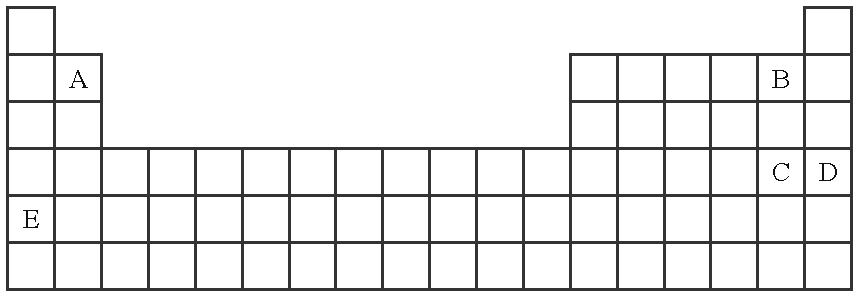
\includegraphics[width=0.6\linewidth]{FigurasSVG/UD2_Tabla_Periodica/pdf/UD2_E01_ejercicio_tabla.pdf}
        \caption{Tabla periódica}
        \label{fig:ejercicio_2}
    \end{figure}
    \begin{solu}
%        \begin{figure}[H]
%            \centering
%            \includegraphics[scale=.5]{ images/imagesUD2TablaPeriodica/UD2_Problemas/evauclm3a.png}
%            \includegraphics[scale=.5]{ images/imagesUD2TablaPeriodica/UD2_Problemas/evauclm3b.png}
%        \end{figure}

        Según su posición en el esquema de la tabla periódica: \(A\) está en el grupo 2, período 2 (berilio, \(Z=4\)); \(B\) está en el grupo 17, período 2 (flúor, \(Z=9\)); \(C\) y \(D\) están al final del período 3, en los grupos 17 y 18 respectivamente (cloro, \(Z=17\), y argón, \(Z=18\)); y \(E\) está en el grupo 1, período 4 (potasio, \(Z=19\)).

        \textbf{Configuraciones electrónicas}

        \begin{itemize}
            \item \(A\) (Be, \(Z=4\)): \(1s^2\,2s^2\)
            \item \(B\) (F, \(Z=9\)): \(1s^2\,2s^2\,2p^5\)
            \item \(C\) (Cl, \(Z=17\)): \(1s^2\,2s^2\,2p^6\,3s^2\,3p^5\)
            \item \(D\) (Ar, \(Z=18\)): \(1s^2\,2s^2\,2p^6\,3s^2\,3p^6\)
            \item \(E\) (K, \(Z=19\)): \(1s^2\,2s^2\,2p^6\,3s^2\,3p^6\,4s^1\)
        \end{itemize}

        Véase el ejercicio siguiente para el análisis razonado de las afirmaciones sobre estos elementos.

    \end{solu}

\end{exerciseEVAU}

\begin{exerciseEVAU}
    \textbf{2018 (continuación)}. Los elementos A, B, C, D y E son los mismos del ejercicio anterior, situados en el esquema de tabla periódica: \(A\) = Be (\(Z=4\)), \(B\) = F (\(Z=9\)), \(C\) = Cl (\(Z=17\)), \(D\) = Ar (\(Z=18\)) y \(E\) = K (\(Z=19\)).
    \begin{enumerate}[label=\letraminuscula]
    \item Escribe las configuraciones electrónicas de dichos elementos.
    \item Basándote en ellas justifica si son o no ciertas las siguientes afirmaciones:
    \begin{enumerate}
        \item La primera energía de ionización de E es mayor que la de A
        \item D es un gas noble y E un metal alcalinotérreo.
        \item La afinidad electrónica de B es mayor que la de A.
        \item El radio atómico de C es mayor que el de B.
    \end{enumerate}
    \end{enumerate}

    \begin{solu}

        \textbf{a) Configuraciones electrónicas}

        \begin{itemize}
            \item \(A\) (Be, \(Z=4\)): \(1s^2\,2s^2\)
            \item \(B\) (F, \(Z=9\)): \(1s^2\,2s^2\,2p^5\)
            \item \(C\) (Cl, \(Z=17\)): \(1s^2\,2s^2\,2p^6\,3s^2\,3p^5\)
            \item \(D\) (Ar, \(Z=18\)): \(1s^2\,2s^2\,2p^6\,3s^2\,3p^6\)
            \item \(E\) (K, \(Z=19\)): \(1s^2\,2s^2\,2p^6\,3s^2\,3p^6\,4s^1\)
        \end{itemize}

        \textbf{b) Análisis de las afirmaciones}

        \textbf{b.1) «La primera energía de ionización de E es mayor que la de A»: FALSO.}

        \(E\) (K) es un metal alcalino del grupo 1, con un único electrón de valencia muy alejado del núcleo (período 4), por lo que su energía de ionización es muy baja. \(A\) (Be) pertenece al grupo 2, con mayor carga nuclear efectiva sobre sus electrones de valencia y en una capa más interna (período 2), lo que le confiere una energía de ionización considerablemente mayor que la de \(E\).

        \textbf{b.2) «D es un gas noble y E un metal alcalinotérreo»: FALSO.}

        \(D\) (Ar) sí es un gas noble (grupo 18), pero \(E\) (K) tiene configuración \(4s^1\), propia de un \textbf{metal alcalino} (grupo 1), no de un metal alcalinotérreo (grupo 2, que tendría configuración \(ns^2\)). Por tanto, la primera parte es cierta, pero la segunda es falsa.

        \textbf{b.3) «La afinidad electrónica de B es mayor que la de A»: VERDADERO.}

        \(B\) (F) tiene mayor carga nuclear (\(Z=9\)) que \(A\) (Be, \(Z=4\)) y, al pertenecer ambos al período 2 con un apantillamiento interno similar, también mayor carga nuclear efectiva \(Z_{ef}\) sobre su capa de valencia. \(B\) es además un halógeno al que solo le falta un electrón para alcanzar la configuración de gas noble, por lo que su afinidad electrónica es muy alta (proceso muy favorable). \(A\) (Be), en cambio, tiene la subcapa \(2s\) completa, una configuración de especial estabilidad que dificulta la entrada de un electrón adicional; su afinidad electrónica es prácticamente nula o incluso desfavorable. Por tanto, la afinidad electrónica de \(B\) es, efectivamente, mayor que la de \(A\).

        \textbf{b.4) «El radio atómico de C es mayor que el de B»: VERDADERO.}

        \(C\) (Cl) y \(B\) (F) pertenecen al mismo grupo (17), pero \(C\) se encuentra en el período 3 y \(B\) en el período 2. Al descender en un grupo, el radio atómico aumenta porque los electrones de valencia ocupan capas cada vez más alejadas del núcleo. Por tanto, el radio de \(C\) es mayor que el de \(B\).

    \end{solu}
\end{exerciseEVAU}

\begin{exerciseEVAU}
    \textbf{2021}.
    A partir de los átomos A (Z =19) y B (Z = 35): a) Escriba sus configuraciones electrónicas, indique el grupo y el periodo al que pertenecen. b) ¿El radio del ion más estable de A es inferior al del ion más estable de B? Justifíquelo. c) ¿Qué se entiende por primera energía de ioniza ión de un átomo? ¿Cuál de los átomos A y B tendría mayor energía de ionización? d) Formule el compuesto binario que podrían formar A y B razonando el tipo de enlace que se generaría.

    \begin{solu}
%        \begin{figure}[H]
%            \centering
%            \includegraphics[scale=.5]{ images/imagesUD2TablaPeriodica/UD2_Problemas/evauclm4.png}
%        \end{figure}

        \textbf{a) Configuraciones electrónicas, grupo y período}

        \begin{itemize}
            \item \(A\) (\(Z=19\), K): \(1s^2\,2s^2\,2p^6\,3s^2\,3p^6\,4s^1\) — grupo 1, período 4.
            \item \(B\) (\(Z=35\), Br): \(1s^2\,2s^2\,2p^6\,3s^2\,3p^6\,4s^2\,3d^{10}\,4p^5\) — grupo 17, período 4.
        \end{itemize}

        \textbf{b) Comparación de los radios iónicos}

        El ion más estable de \(A\) es \(\ch{K+}\) (pierde su único electrón de valencia y adquiere la configuración del \ch{Ar}, con capa de valencia \(n=3\)). El ion más estable de \(B\) es \(\ch{Br-}\) (gana un electrón y adquiere la configuración del \ch{Kr}, con capa de valencia \(n=4\)).

        Como \(\ch{Br-}\) tiene su capa de valencia en \(n=4\) (más externa) y muchos más electrones que \(\ch{K+}\) (36 frente a 18), su radio es considerablemente mayor: la mayor extensión de la nube electrónica prevalece sobre el hecho de que la carga nuclear de \(\ch{Br-}\) (\(Z=35\)) sea mayor que la de \(\ch{K+}\) (\(Z=19\)). Por tanto, \textbf{sí}, el radio de \(\ch{K+}\) es inferior al de \(\ch{Br-}\).

        \textbf{c) Primera energía de ionización}

        La primera energía de ionización es la energía necesaria para arrancar el electrón más externo (el menos retenido) a un átomo aislado en estado fundamental y gaseoso, dando lugar a un catión monopositivo.

        Entre \(A\) y \(B\), el bromo (\(B\)) tiene mayor carga nuclear (\(Z=35\)) y, al ser un no metal próximo a la configuración de gas noble, una elevada carga nuclear efectiva \(Z_{ef}\) sobre sus electrones de valencia, por lo que los retiene con mucha más fuerza que el potasio (\(A\)), un metal alcalino con un único electrón de valencia muy alejado del núcleo y muy apantallado (\(Z_{ef}\) baja). Por tanto, \(\boldsymbol{B}\) \textbf{(Br) tiene mayor energía de ionización}.

        \textbf{d) Compuesto binario entre A y B}

        El potasio (metal muy electropositivo) cede su electrón de valencia al bromo (no metal muy electronegativo), formando el compuesto iónico:

        \begin{equation*}
            \ch{KBr}
        \end{equation*}

        (bromuro de potasio), unido mediante \textbf{enlace iónico}.

    \end{solu}
\end{exerciseEVAU}


\begin{exerciseEVAU}
    \textbf{2017}. Los átomos neutros A, B, C y D tienen las siguientes configuraciones electrónicas: $A = 1s^2 2s^2 2p^1$; $B = 1s^2 2s^2 2p^5$; $C = 1s^2 2s^2 2p^6 3s^2$; $D = 1s^2 2s^2 2p^6$
    a) Indica el grupo y período en el que se encuentran.
    b) El nombre y símbolo de cada elemento
    c) Ordena razonadamente, de mayor a menor electronegatividad.
    d) ¿Cuál de ellos presentará mayor potencial de ionización?

    \begin{solu}
%        \begin{figure}[H]
%            \centering
%            \includegraphics[scale=.5]{ images/imagesUD2TablaPeriodica/UD2_Problemas/evauclm3a.png}
%        \end{figure}

        A partir de las configuraciones electrónicas dadas, identificamos cada elemento: \(A\) tiene 5 electrones (\(Z=5\), boro), \(B\) tiene 9 electrones (\(Z=9\), flúor), \(C\) tiene 12 electrones (\(Z=12\), magnesio) y \(D\) tiene 10 electrones (\(Z=10\), neón).

        \textbf{a) Grupo y período}

        \begin{itemize}
            \item \(A\) (B, \(Z=5\)): grupo 13, período 2.
            \item \(B\) (F, \(Z=9\)): grupo 17, período 2.
            \item \(C\) (Mg, \(Z=12\)): grupo 2, período 3.
            \item \(D\) (Ne, \(Z=10\)): grupo 18, período 2.
        \end{itemize}

        \textbf{b) Nombre y símbolo}

        \(A\) = boro (\ch{B}); \(B\) = flúor (\ch{F}); \(C\) = magnesio (\ch{Mg}); \(D\) = neón (\ch{Ne}).

        \textbf{c) Orden de mayor a menor electronegatividad}

        El flúor es el elemento más electronegativo de toda la tabla periódica. El magnesio, al ser un metal, tiene una electronegatividad baja. El neón, al ser un gas noble prácticamente inerte, no forma enlaces en condiciones normales y carece de un valor de electronegatividad de Pauling definido (o se considera nulo a estos efectos). Entre los elementos con electronegatividad definida:

        \begin{equation*}
            B\,(\ch{F}) > A\,(\ch{B}) > C\,(\ch{Mg})
        \end{equation*}

        \textbf{d) Elemento con mayor potencial de ionización}

        Los cuatro elementos pertenecen al período 2, por lo que el apantallamiento interno es similar para todos ellos y la carga nuclear efectiva \(Z_{ef} = Z - \sigma\) aumenta con el número atómico: \(D\) (Ne, \(Z=10\)) tiene la mayor \(Z_{ef}\) del grupo. \(D\) (neón) presenta el mayor potencial de ionización, ya que posee configuración de capa cerrada (gas noble), de especial estabilidad, lo que, junto con su elevada carga nuclear efectiva, dificulta enormemente arrancarle un electrón.

    \end{solu}
\end{exerciseEVAU}


